% !Mode:: "TeX:UTF-8" 

\chapter{示例文档}[Example]

这是 \hithesis\ 的示例文档,基本上覆盖了模板中所有格式的设置。建议大家在使用模板
之前,除了阅读《\hithesis\ 用户手册》,这个示例文档也最好能看一看。

\section{索引示例}[Index]

折腾了这久,月亮已渐到中天,段誉迳向西行,他虽不会武功,但年轻力壮,脚下也甚迅捷
,走出十余里,已经到无量山峰的后山,只听得水声淙淙,前面有条山溪。他正感口渴,寻
\sindex[china]{qi!乔峰}声来到溪旁,月光下溪水清澈异常,刚伸手入溪,忽听得远处地
下枯枝格的一响,跟着有两\sindex[english]{Xu Zhu}人的脚步之声,段誉忙俯伏溪边,不
敢稍动。\sindex[english]{Qiao Feng}

\subsection{引用}[Cite]
\sindex[china]{du!段誉}中又有两乘分道而行。段誉心知鸠摩智意在扰乱追兵,叫他们不
知向何处追赶才是\cite{cnproceed}。再奔得一阵,鸠摩智跃下马背,取过一根皮带,缚在
段誉腰间,左手提着他身子,便从山坳里行去\inlinecite{hithesis2017},另外两名汉子
却纵马西驰。段誉暗暗叫苦,心道:“伯父便派遣铁甲骑兵不停追赶,至多也不过将这番僧
的九名随从尽数擒去,可救我不得\cite{cnarticle}。

\subsection{图片}[Pictures]
\subsubsection{博士毕业论文双语题注}[Doctoral picture example]
段誉受无量剑和神农帮欺凌、为南海鳄神逼迫、被延庆太子囚禁、给鸠摩智俘虏、在曼
陀山庆当花匠种花,所经历的种种苦楚折辱着实不小,但从未有如此刻这般的怨愤气恼。
\begin{figure}[htpb]
\centering
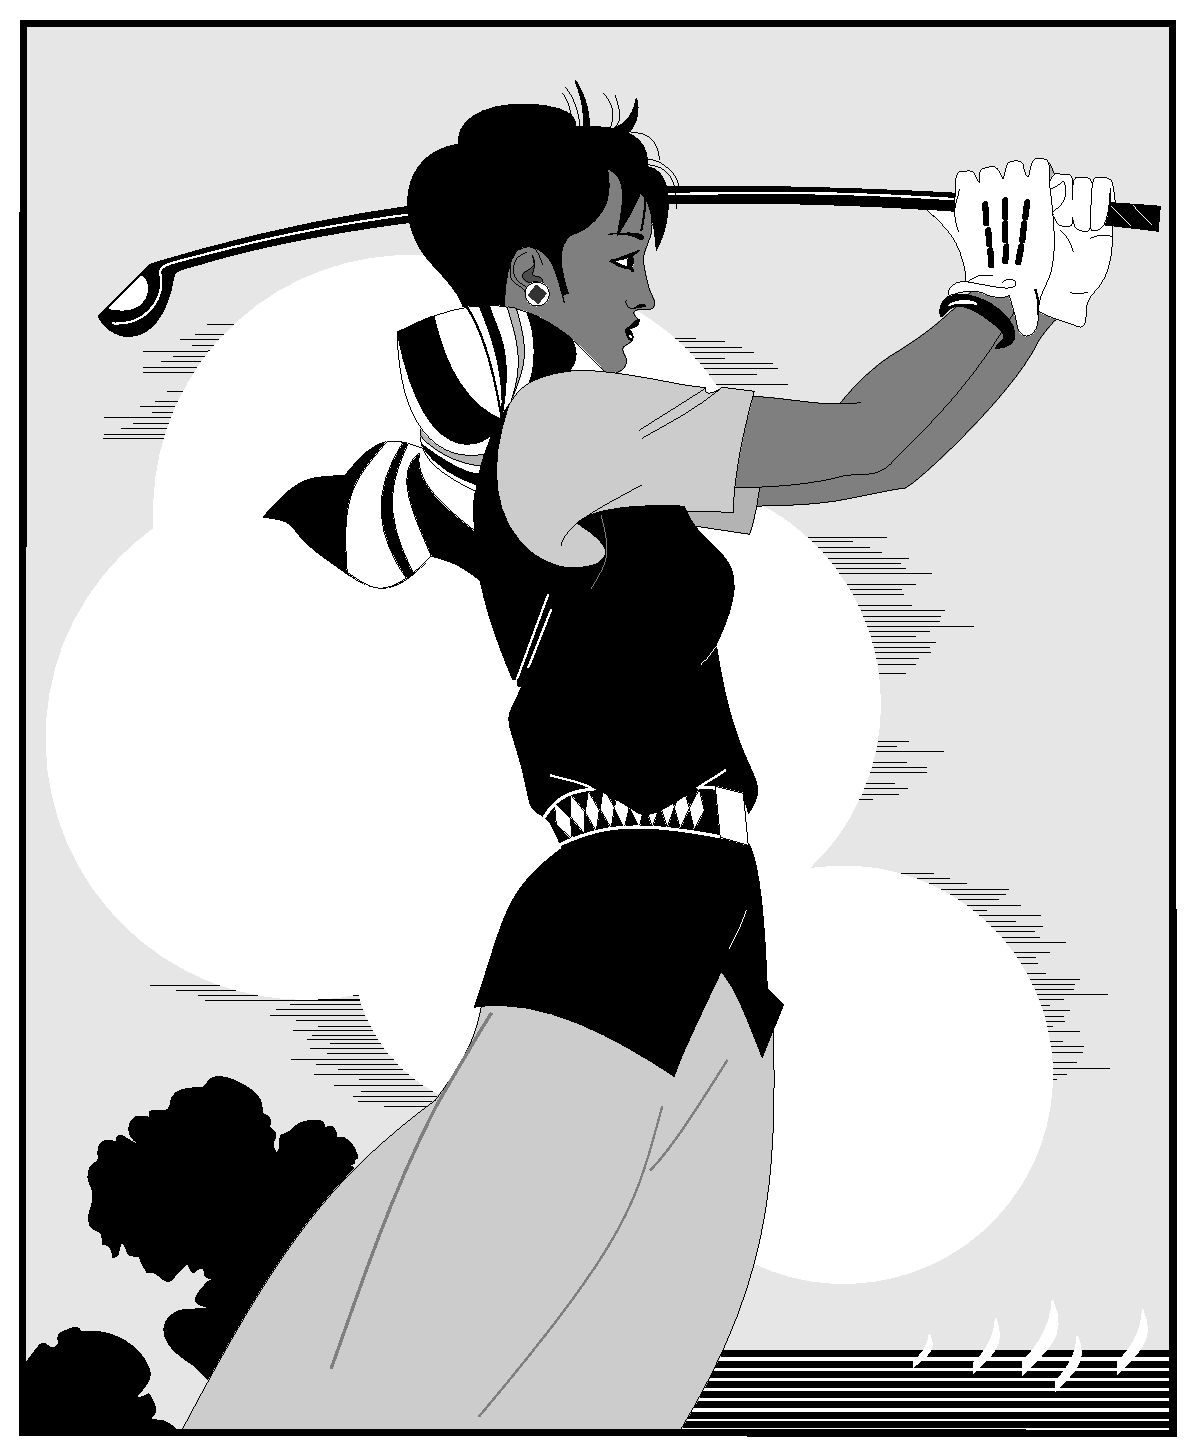
\includegraphics[width = 0.4\textwidth]{golfer}
\bicaption[golfer1]{}{图打打高尔夫球的人打高尔夫球的人打高尔夫球的人打高尔夫球球的人高尔夫球的人球的人高尔夫球的人的人高尔夫球的人}{Fig.$\!$}{The person playing golf playing golf playing golf playing golf playing golf playing golf playing golf playing golf}
\end{figure}
湖上晚风阵阵,带着菱叶清香。段誉用力扳桨,不知要恨谁才好,他实在说不出为什么
这样气恼。当日木婉清、南海鳄神、延庆太子、鸠摩智、王夫人等给他的凌辱,可都厉害得
多了,但他泰然而受,并没感到太大的委屈。

\subsubsection{本硕论文题注}[Other picture example]
他内心隐隐约约的觉得,只因为他深慕王语嫣,而这位姑娘心中,却全没他段誉的半点
影子,甚至阿朱、阿碧,也没当他是一回事。他从小便给人当作心肝宝贝,自大理国皇帝、
皇后以下,没一个不觉得他是了不起之至。就算遇上了敌人,南海鳄神是一心一意的要收他
为徒;鸠摩智不辞辛劳的从大理掳他来到江南,自也对他颇为重视,至于钟灵、木婉清那些
少女,更是一见他便即倾心。
\begin{figure}[h]
\centering
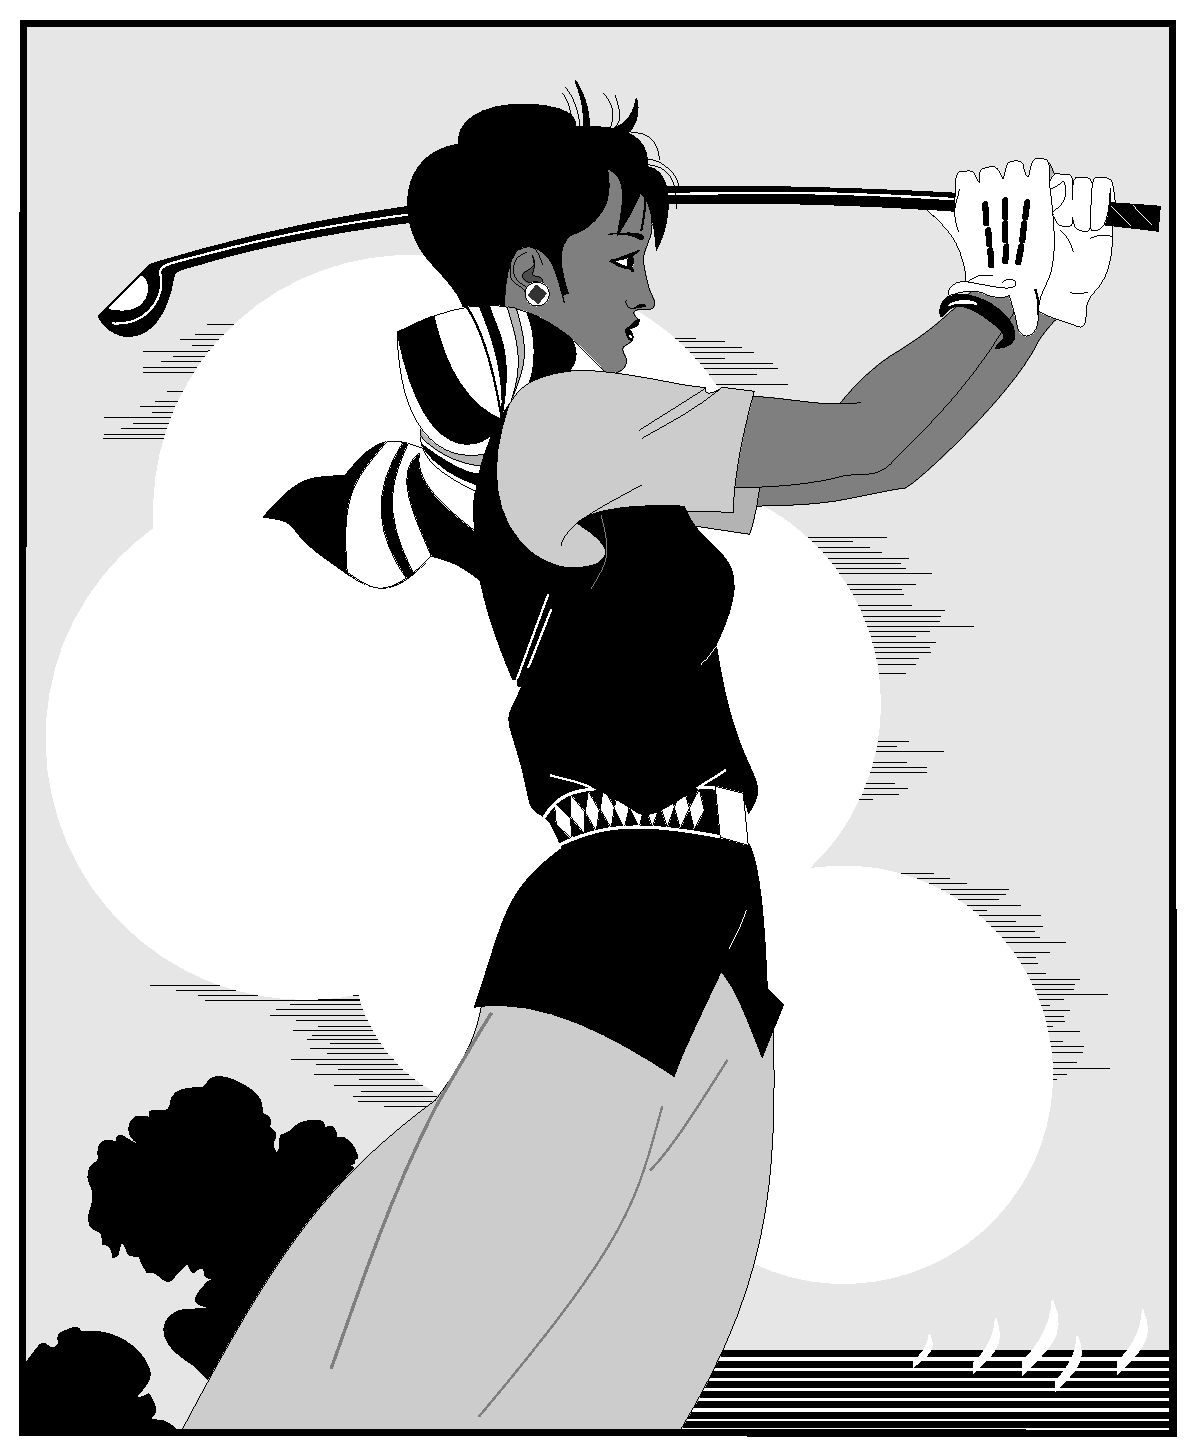
\includegraphics[width = 0.4\textwidth]{golfer}
\caption{图打高高尔夫球的高尔夫球的高尔夫球的高尔夫球的高尔夫球的高尔夫球的高尔夫球的高尔夫球的高尔夫球的高尔夫球的高尔夫球的高尔夫球的高尔夫球的高尔夫球的高尔夫球的高尔夫球的高尔夫球的高尔夫球的高尔夫球的高尔夫球的高尔夫球的高尔夫球的高尔夫球的高尔夫球的注意,这里是模板自动选择最佳字号}
\end{figure}
他一生中从未受过今日这般的冷落轻视,别人虽然有礼,却是漠不关心的有礼。在旁人
心目中,慕容公子当然比他重要得多,这些日子来,只要有谁提到慕容公子,立时便人人耸
动,无不全神贯注的倾听。王语嫣、阿朱、阿碧、包不同,以至什么邓大爷、公冶二爷、风
四爷,个个都似是为慕容公子而生。

\subsubsection{并排图和子图}[Sub-picture example]
那大汉左手将乔峰挟在肋下,长绳甩出,已卷住了大门外聚贤庄高高的旗杆。群雄大声呼喊
,霎时之间钢镖、袖箭、飞刀、铁锥、飞蝗石、甩手箭,各种各样暗器都向乔峰和那大汉身
上射去。那黑衣碜汉一拉长绳,悠悠飞起,往旗杆的旗斗中落去。腾腾、拍拍、擦擦,响声
不绝,数十年暗器都打在旗斗上。只见长绳从旗斗中甩出,绕向八九丈外的一株大树,那大
汉挟着乔峰,从旗斗中荡出,顷刻间越过那株大树,已在离旗杆十科丈处落地。他跟着又甩
长绳,再绕远处大树,如此几个起落,已然走得无影无踪。

\begin{figure}[htbp]
\centering
\begin{minipage}{0.4\textwidth}
\centering
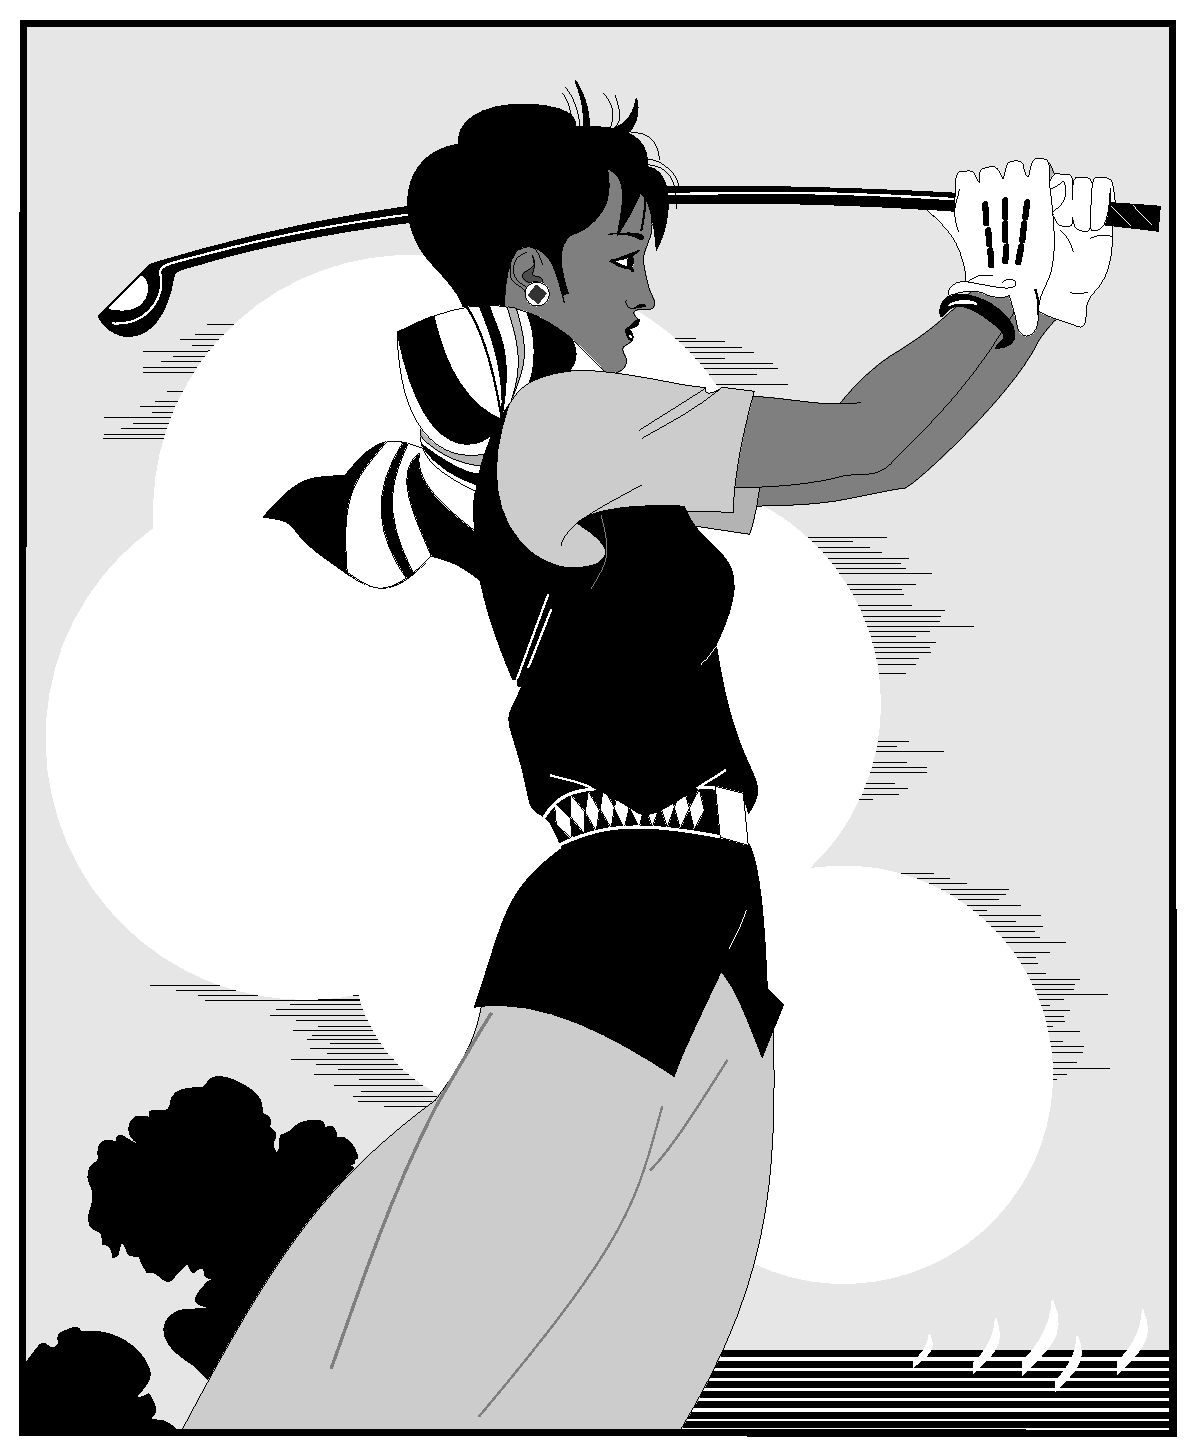
\includegraphics[width=\textwidth]{golfer}
\bicaption[golfer2]{}{打高尔夫球的人}{Fig.$\!$}{The person playing golf}
\end{minipage}
\begin{minipage}{0.4\textwidth}
\centering
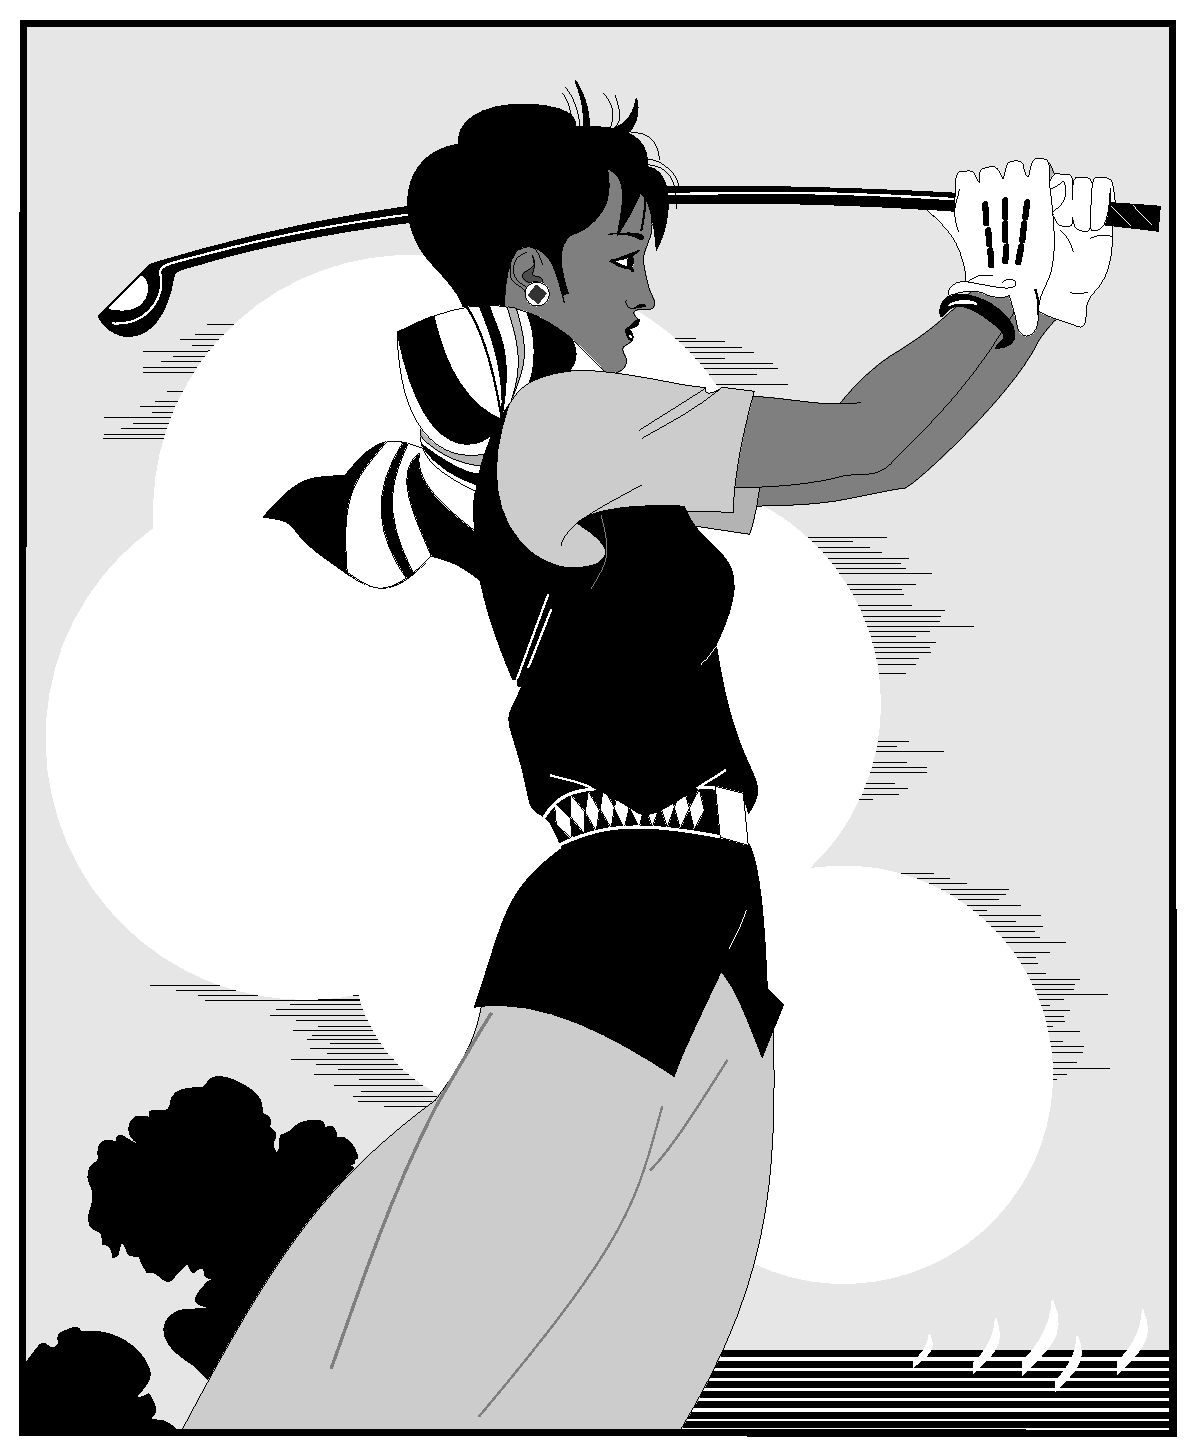
\includegraphics[width=\textwidth]{golfer}
\bicaption[golfer3]{}{打高尔夫球的人}{Fig.$\!$}{The person playing golf}
\end{minipage}
\end{figure}

群雄骇然相顾,但听得马蹄声响,渐驰渐远,再也追不上了。

乔峰受伤虽重,神智未失,这大汉以长绳救他脱险,一举一动,他都看得清清楚楚,自是深
感他救命之恩,又想:“这甩绳的准头膂力,我也能办到,但以长绳当作兵刃,同时挥击数
十人,这一招‘天女散花’的软鞭功夫,我就不能使得如他这般恰到好处。”

那黑衣大汉将他放上马背,两人一骑,径向北行。那大汉取出金创药来,敷上乔峰三处伤口
。乔峰流血过多,虚弱之极,几次都欲晕去,每次都是吸一口气,内息流转,精神便是一振
。那大汉纵马直向西北,走了一会,道路越来越崎岖,到后来已无道路,那马尽是在乱石堆
中踬蹶而行。

\begin{figure}[!h]
\centering
\subfigure{\label{golfer41}}\addtocounter{subfigure}{-2}
\subfigure[The person playing golf]{\subfigure[打高尔夫球的人~1]{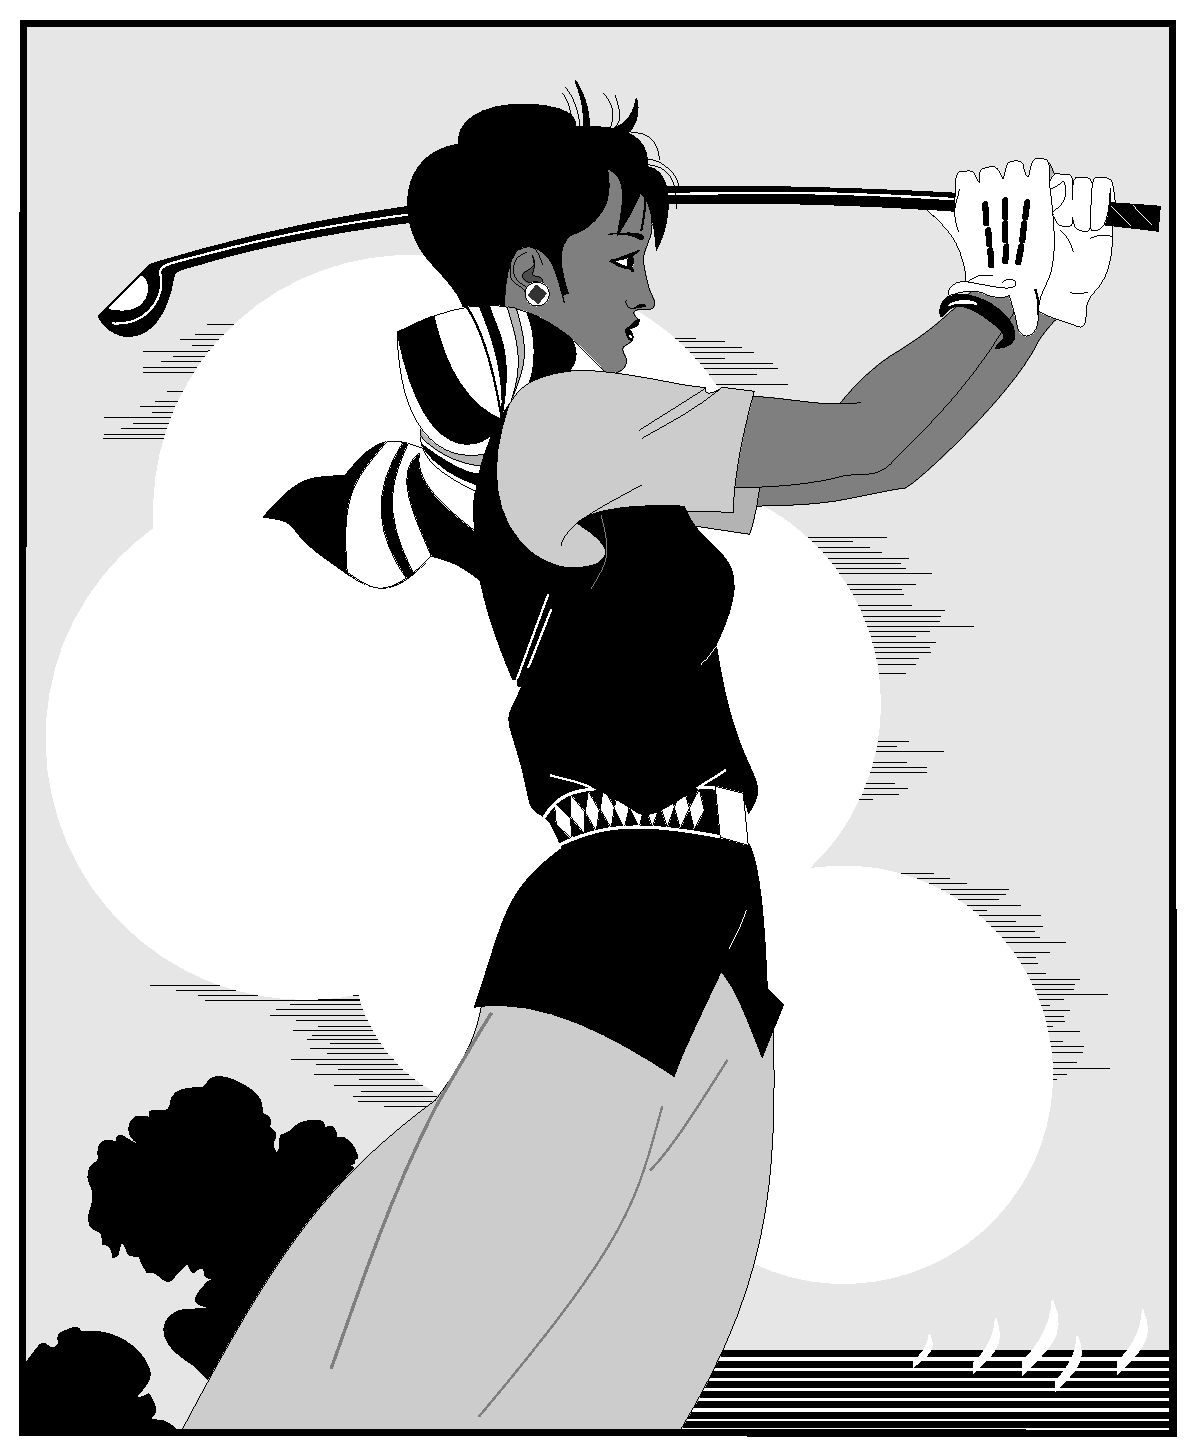
\includegraphics[width=0.4\textwidth]{golfer}}}
\subfigure{\label{golfer42}}\addtocounter{subfigure}{-2}
\subfigure[The person playing golf]{\subfigure[打高尔夫球的人~2]{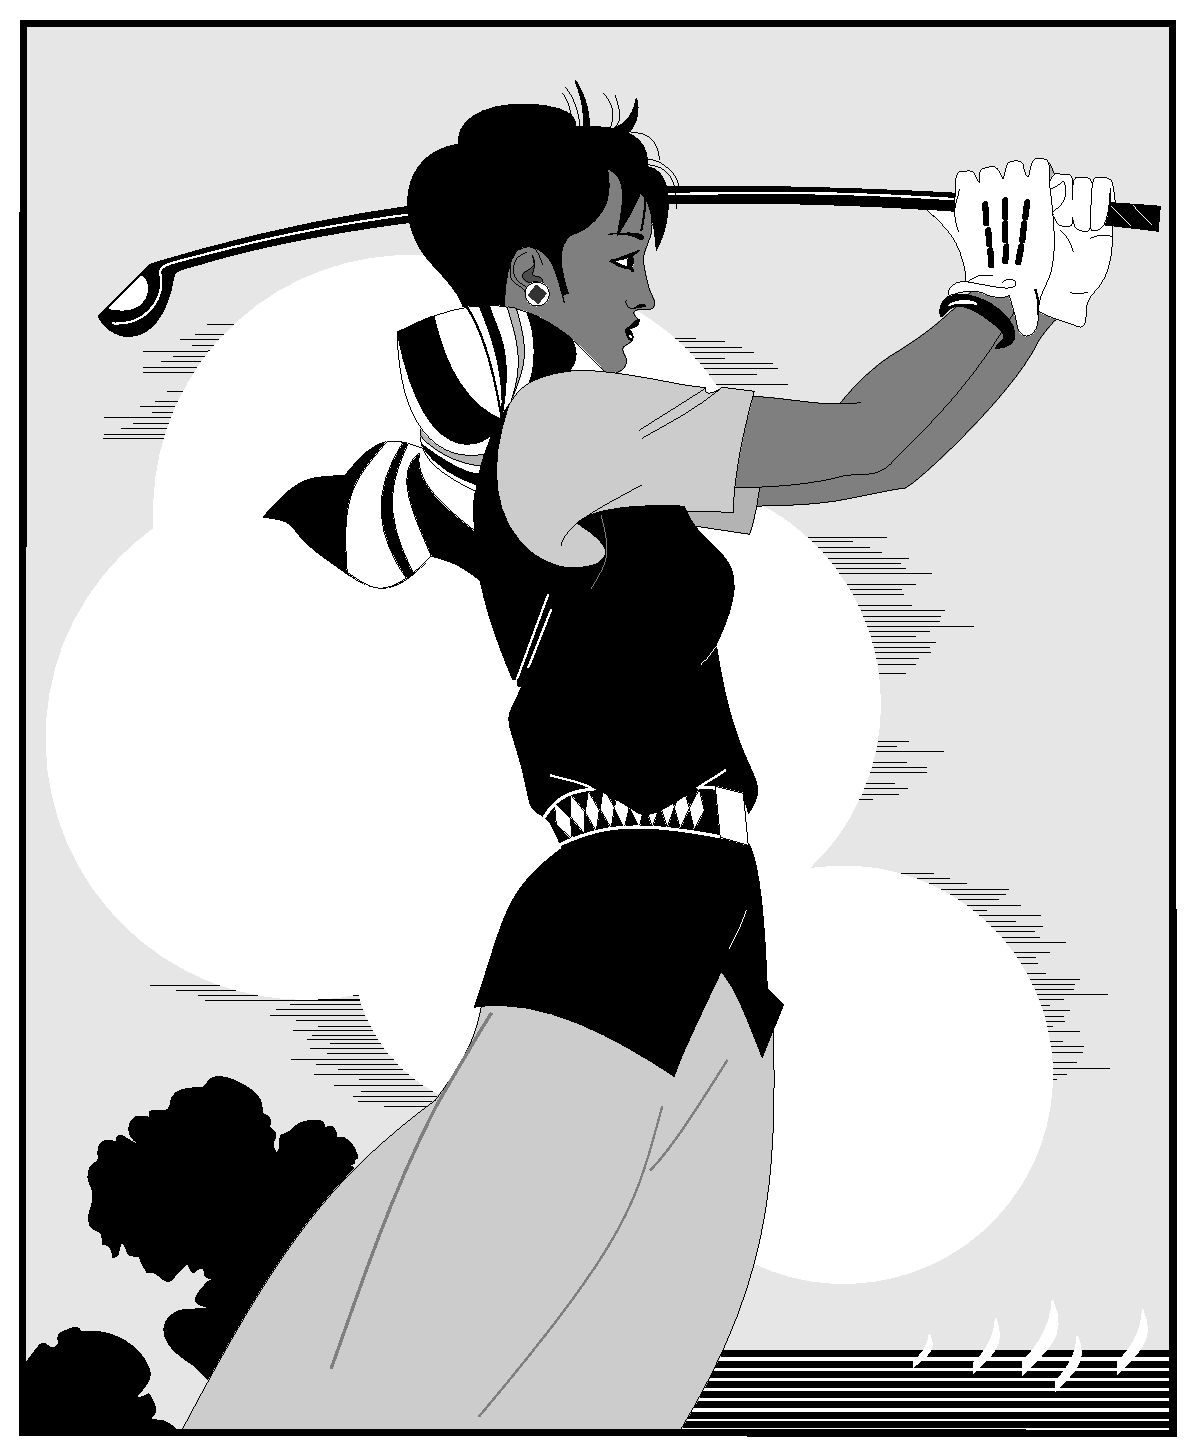
\includegraphics[width=0.4\textwidth]{golfer}}}
\subfigure{\label{golfer43}}\addtocounter{subfigure}{-2}
\subfigure[The person playing golf]{\subfigure[打高尔夫球的人~3]{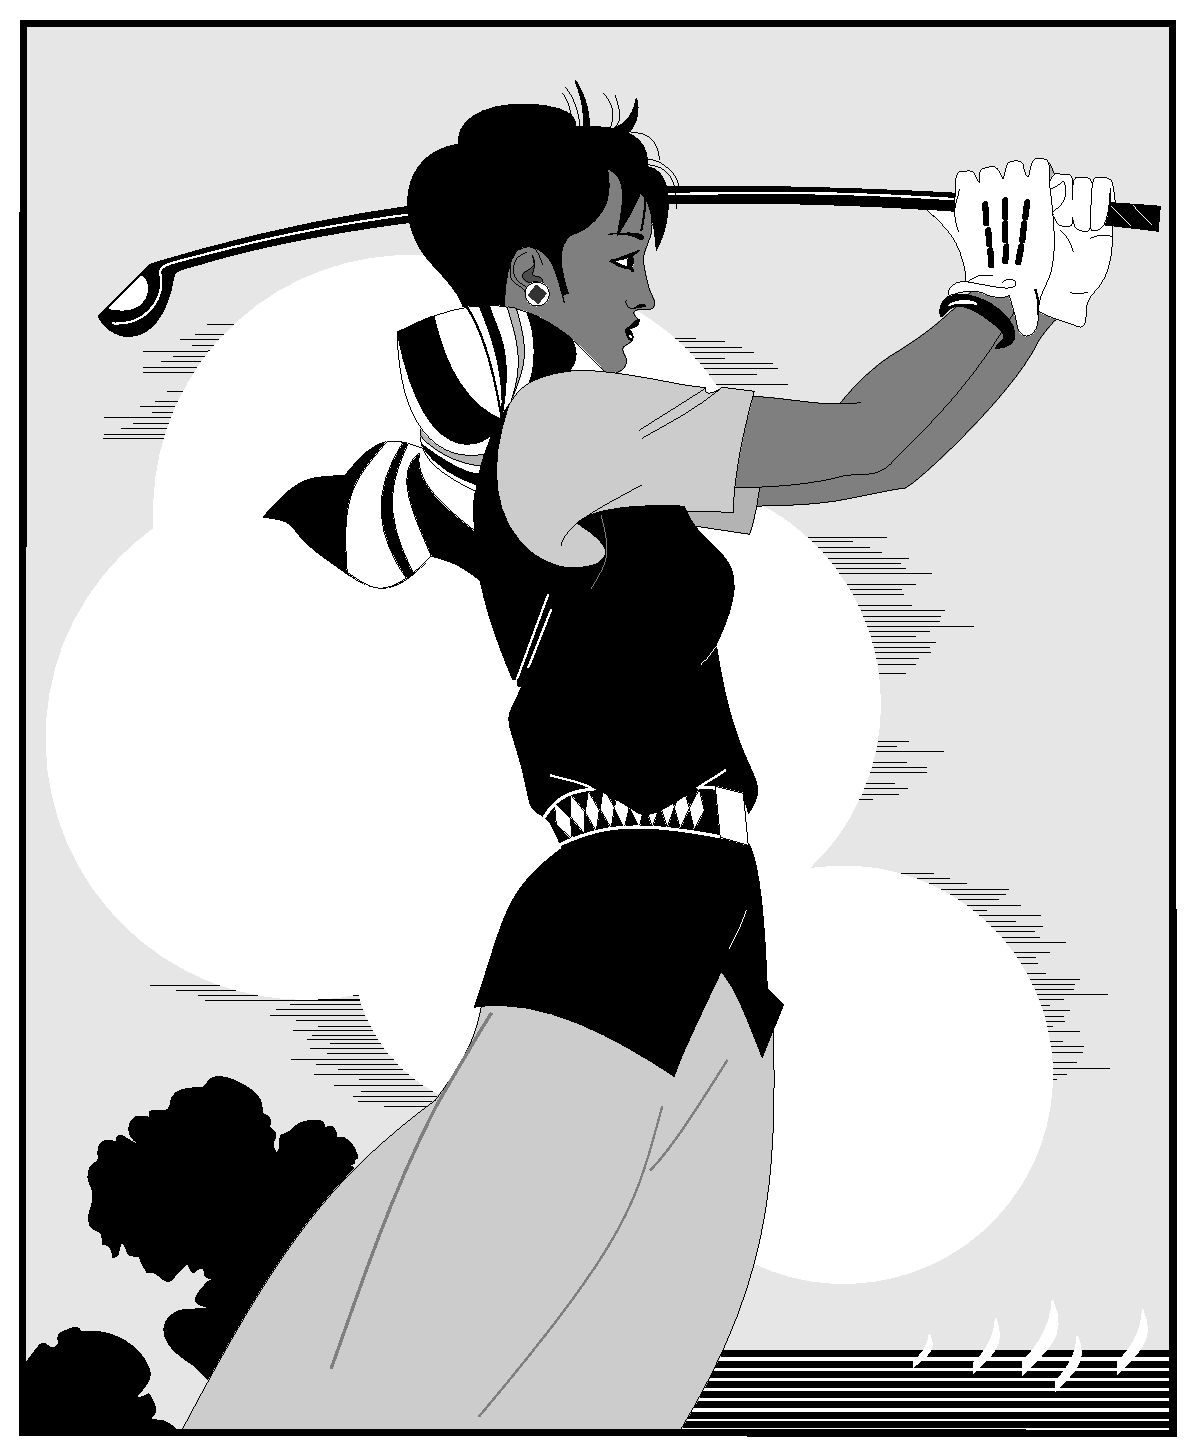
\includegraphics[width=0.4\textwidth]{golfer}}}
\subfigure{\label{golfer44}}\addtocounter{subfigure}{-2}
\subfigure[The person playing golf]{\subfigure[打高尔夫球的人~4]{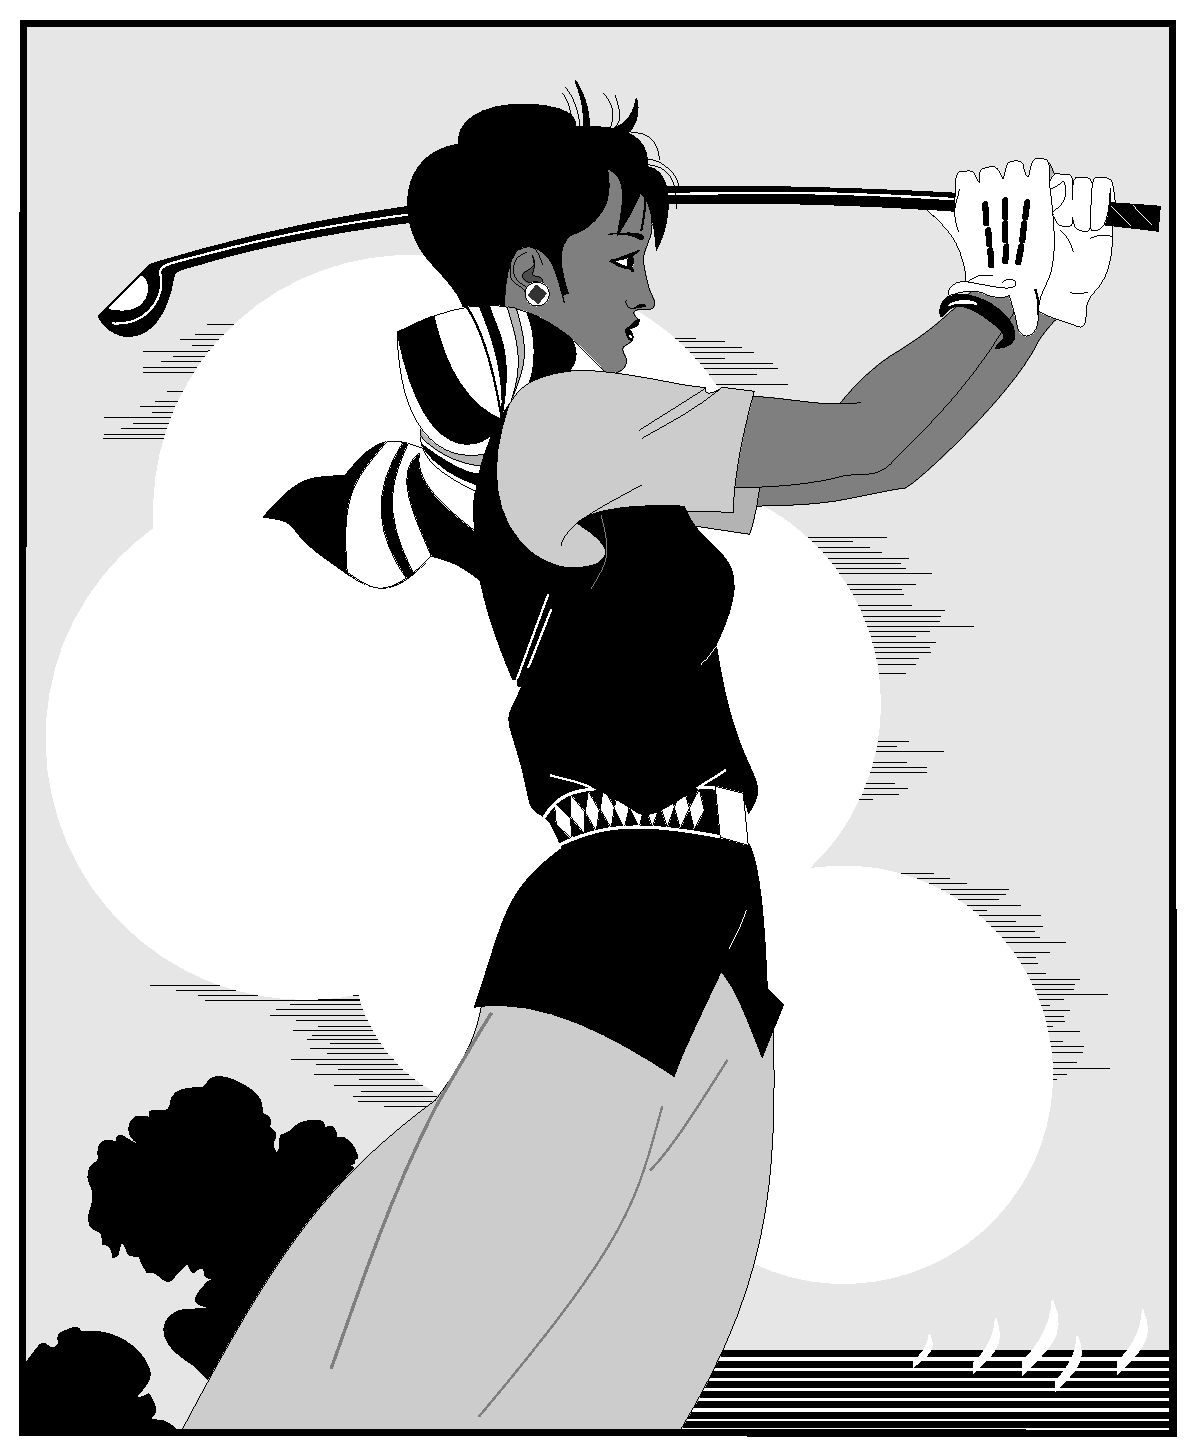
\includegraphics[width=0.4\textwidth]{golfer}}}
\bicaption[golfer4]{}{打高尔夫球的人}{Fig.$\!$}{The person playing golf}
\end{figure}

又行了半上多时辰,马匹再也不能走了,那大汉将乔峰横抱手中,下马向一认山峰上攀去。
乔峰身子甚重,那大汉抱着他却似毫不费力,虽在十分陡峭之处,那大汉便用长绳飞过山峡
,缠住树枝而跃将过去。那人接连横越了八处险峡,跟着一路向下,深入一个上不见天的深
保之中,终于站定脚步,将乔峰放下。

乔峰勉力站定,说道:“大恩不敢言谢,只求恩兄让乔峰一见庐山直面。”

那大汉一对晶光灿然的眼光在他脸上转来转去,过得半晌,说道:“山洞中有足用半月的干
粮,你在此养伤,敌从无法到来。”

乔峰应道:“是!”心道:“听这人声音,似乎年纪不轻了。”

那大汉又向他打量了一会,忽然右手挥出,拍的一声,打了他一记耳光。这一下出手奇快,
乔峰一来绝没想到他竟会击打自己,二来这一掌也当真打得高明之极,竟然没能避开。

那大汉第二记跟着打来,两掌之间,相距只是电光般的一闪,乔峰有了这个余裕,却哪能再
让他打中?但他是救命恩人,不愿跟他对敌,而又无力闪身相避,于是左手食指伸出,放在
自己颊边,指着他的掌心。

这食指所向,是那大汉掌心的“劳宫穴”,他一掌拍将过来,手掌未及乔峰面颊,自己掌上要
实先得碰到手指。这大汉手掌离乔峰面颊不到一尺,立即翻掌,用手背向他击去,这一下变
招奇速。乔峰也是迅速之极的转过手指,指尖对住了他手背上的“二间穴”。

那大汉一声长笑,右手硬生生的缩回,左手横斩而至。乔峰左手手指伸出,指尖已对准他掌
缘的“后豁穴”。那大汉手臂陡然一提,来势不衰,乔峰及时移指,指向耸掌缘的“前谷穴”。
顷刻之间,那大汉双掌飞舞,连换了十余下招式,乔峰只守不攻,手指总是指着他手掌击来
定会撞上的穴道。那大汉第一下出其不意的打了他一记巴掌,此后便再也打他不着了。两从
虚发虚接,个是当世罕见的上乘武功。

那大汉使满第二十招,见乔峰虽在重伤之余,仍是变招奇快,认穴奇准,陡然间收掌后跃,
说道:“你这人愚不中及,我本来不该救你。”乔峰道:“谨领恩公教言。”

那人骂道:“你这臭骡子,练就了这样一身天下无敌的武功,怎地去为一上瘦骨伶仃的女娃
子枉送性命?她跟你非亲非故,无恩无义,又不是什么倾国倾城的美貌佳人,只不过是一个
低三下四的小丫头而已。天下哪有你这等大傻瓜?”

乔峰叹了口气,说道:“恩公教训得是。乔峰以有用之身,为此无益之事,原是不当。只是
一时气愤难当,蛮劲发作,便没细想后果。”

那大汉道:“嘿嘿,原来是蛮劲发作。”抬头向天,纵声长笑。

乔峰只觉他长笑声中大有悲凉愤慨之意,不禁愕然。蓦地里见那大汉拔身而起,跃出丈余,
身形一晃,已在一块大岩之后隐没。乔峰叫道:“恩公,恩公!”但见他接连纵跃,转过山峡
,竟远远的去了。乔峰只跨出一步,便摇摇欲倒,忙伸手扶住山壁。

\section{表格}

表应有自明性。表格不加左、右边线。表的编排建议采用国际通行的三线表。表中文字用宋
体~5~号字。每个表格均应有表题(由表序和表名组成)。表序一般按章编排,如第~1~章第
一个插表的序号为“表~1-1”等。表序与表名之间空一格,表名中不允许使用标点符号,表名
后不加标点。表题置于表上,硕士学位论文只用中文,博士学位论文用中、英文两种文字居
中排写,中文在上,要求中文用宋体~5~号字,英文用新罗马字体~5~号字。表头设计应简单
明了,尽量不用斜线。表头中可采用化学符号或物理量符号。


\subsection{普通表格的绘制方法}[Methods of drawing normal tables]

表格应具有三线表格式,因此需要调用~booktabs~宏包,其标准格式如表~\ref{table1}~所示。
\begin{table}[htbp]
\bicaption[table1]{}{符合研究生院绘图规范的表格}{Table$\!$}{Table in agreement of the standard from graduate school}
\vspace{0.5em}\centering\wuhao
\begin{tabular}{ccccc}
\toprule[1.5pt]
$D$(in) & $P_u$(lbs) & $u_u$(in) & $\beta$ & $G_f$(psi.in)\\
\midrule[1pt]
 5 & 269.8 & 0.000674 & 1.79 & 0.04089\\
10 & 421.0 & 0.001035 & 3.59 & 0.04089\\
20 & 640.2 & 0.001565 & 7.18 & 0.04089\\
\bottomrule[1.5pt]
\end{tabular}
\end{table}
全表如用同一单位,则将单位符号移至表头右上角,加圆括号。表中数据应准确无误,书写
清楚。数字空缺的格内加横线“-”(占~2~个数字宽度)。表内文字或数字上、下或左、右
相同时,采用通栏处理方式,不允许用“〃”、“同上”之类的写法。表内文字说明,起行空一
格、转行顶格、句末不加标点。如某个表需要转页接排,在随后的各页上应重复表的编号。
编号后加“(续表)”,表题可省略。续表应重复表头。

\subsection{长表格的绘制方法}[Methods of drawing long tables]

长表格是当表格在当前页排不下而需要转页接排的情况下所采用的一种表格环境。若长表格
仍按照普通表格的绘制方法来获得,其所使用的\verb|table|浮动环境无法实现表格的换页
接排功能,表格下方过长部分会排在表格第1页的页脚以下。为了能够实现长表格的转页接
排功能,需要调用~longtable~宏包,由于长表格是跨页的文本内容,因此只需要单独的
\verb|longtable|环境,所绘制的长表格的格式如表~\ref{table2}~所示。

注意,长表格双语标题的格式。

\ltfontsize{\dawu[1.667]}
\dawu[1.667]\begin{longtable}{ccc}%
\longbionenumcaption{}{{\wuhao 中国省级行政单位一览
}\label{table2}}{Table$\!$}{}{{\wuhao Overview of the provincial administrative
unit of China}}{-0.5em}{3.15bp}\\
%\caption{\wuhao 中国省级行政单位一览}\\
\toprule[1.5pt] 名称 & 简称 & 省会或首府  \\ \midrule[1pt]
\endfirsthead
\multicolumn{3}{r}{表~\thetable(续表)}\vspace{0.5em}\\
\toprule[1.5pt] 名称 & 简称 & 省会或首府  \\ \midrule[1pt]
\endhead
\bottomrule[1.5pt]
\endfoot
北京市 & 京 & 北京\\
天津市 & 津 & 天津\\
河北省 & 冀 & 石家庄市\\
山西省 & 晋 & 太原市\\
内蒙古自治区 & 蒙 & 呼和浩特市\\
辽宁省 & 辽 & 沈阳市\\
吉林省 & 吉 & 长春市\\
黑龙江省 & 黑 & 哈尔滨市\\
上海市 & 沪/申 & 上海\\
江苏省 & 苏 & 南京市\\
浙江省 & 浙 & 杭州市\\
安徽省 & 皖 & 合肥市\\
福建省 & 闽 & 福州市\\
江西省 & 赣 & 南昌市\\
山东省 & 鲁 & 济南市\\
河南省 & 豫 & 郑州市\\
湖北省 & 鄂 & 武汉市\\
湖南省 & 湘 & 长沙市\\
广东省 & 粤 & 广州市\\
广西壮族自治区 & 桂 & 南宁市\\
海南省 & 琼 & 海口市\\
重庆市 & 渝 & 重庆\\
四川省 & 川/蜀 & 成都市\\
贵州省 & 黔/贵 & 贵阳市\\
云南省 & 云/滇 & 昆明市\\
西藏自治区 & 藏 & 拉萨市\\
陕西省 & 陕/秦 & 西安市\\
甘肃省 & 甘/陇 & 兰州市\\
青海省 & 青 & 西宁市\\
宁夏回族自治区 & 宁 & 银川市\\
新疆维吾尔自治区 & 新 & 乌鲁木齐市\\
香港特别行政区 & 港 & 香港\\
澳门特别行政区 & 澳 & 澳门\\
台湾省 & 台 & 台北市\\
\end{longtable}\normalsize

\ltfontsize{\dawu[1.667]}
\dawu[1.667]\begin{longtable}{ccc}%
  \caption{\wuhao 中国省级行政单位一览}\\[0.3em]
\toprule[1.5pt] 名称 & 简称 & 省会或首府  \\ \midrule[1pt]
\endfirsthead
\multicolumn{3}{r}{表~\thetable(续表)}\vspace{0.5em}\\
\toprule[1.5pt] 名称 & 简称 & 省会或首府  \\ \midrule[1pt]
\endhead
\bottomrule[1.5pt]
\endfoot
北京市 & 京 & 北京\\
天津市 & 津 & 天津\\
河北省 & 冀 & 石家庄市\\
山西省 & 晋 & 太原市\\
内蒙古自治区 & 蒙 & 呼和浩特市\\
辽宁省 & 辽 & 沈阳市\\
吉林省 & 吉 & 长春市\\
黑龙江省 & 黑 & 哈尔滨市\\
上海市 & 沪/申 & 上海\\
江苏省 & 苏 & 南京市\\
浙江省 & 浙 & 杭州市\\
安徽省 & 皖 & 合肥市\\
福建省 & 闽 & 福州市\\
江西省 & 赣 & 南昌市\\
山东省 & 鲁 & 济南市\\
河南省 & 豫 & 郑州市\\
湖北省 & 鄂 & 武汉市\\
湖南省 & 湘 & 长沙市\\
广东省 & 粤 & 广州市\\
广西壮族自治区 & 桂 & 南宁市\\
海南省 & 琼 & 海口市\\
重庆市 & 渝 & 重庆\\
四川省 & 川/蜀 & 成都市\\
贵州省 & 黔/贵 & 贵阳市\\
云南省 & 云/滇 & 昆明市\\
西藏自治区 & 藏 & 拉萨市\\
陕西省 & 陕/秦 & 西安市\\
甘肃省 & 甘/陇 & 兰州市\\
青海省 & 青 & 西宁市\\
宁夏回族自治区 & 宁 & 银川市\\
新疆维吾尔自治区 & 新 & 乌鲁木齐市\\
香港特别行政区 & 港 & 香港\\
澳门特别行政区 & 澳 & 澳门\\
台湾省 & 台 & 台北市\\
\end{longtable}\normalsize
此长表格~\ref{table2}~第~2~页的标题“编号(续表)”和表头是通过代码自动添加上去的,无需人工添加,若表格在页面中的竖直位置发生了变化,长表格在第~2~页
及之后各页的标题和表头位置能够始终处于各页的最顶部,也无需人工调整,\LaTeX~系统的这一优点是~word~等软件所无法比拟的。

\subsection{列宽可调表格的绘制方法}[Methods of drawing tables with adjustable-width columns]
论文中能用到列宽可调表格的情况共有两种,一种是当插入的表格某一单元格内容过长以至
于一行放不下的情况,另一种是当对公式中首次出现的物理量符号进行注释的情况,这两种
情况都需要调用~tabularx~宏包。下面将分别对这两种情况下可调表格的绘制方法进行阐述
。
\subsubsection{表格内某单元格内容过长的情况}{The condition when the contents in some cells of tables are too long}
首先给出这种情况下的一个例子如表~\ref{table3}~所示。
\begin{table}[htbp]
  \centering
\bicaption[table3]{}{最小的三个正整数的英文表示法}{Table$\!$}{The English construction of the smallest three positive integral numbers}\vspace{0.5em}\wuhao
\begin{tabularx}{0.7\textwidth}{llX}
\toprule[1.5pt]
Value & Name & Alternate names, and names for sets of the given size\\\midrule[1pt]
1 & One & ace, single, singleton, unary, unit, unity\\
2 & Two & binary, brace, couple, couplet, distich, deuce, double, doubleton, duad, duality, duet, duo, dyad, pair, snake eyes, span, twain, twosome, yoke\\
3 & Three & deuce-ace, leash, set, tercet, ternary, ternion, terzetto, threesome, tierce, trey, triad, trine, trinity, trio, triplet, troika, hat-trick\\\bottomrule[1.5pt]
\end{tabularx}
\end{table}
tabularx环境共有两个必选参数:第1个参数用来确定表格的总宽度,第2个参数用来确定每
列格式,其中标为X的项表示该列的宽度可调,其宽度值由表格总宽度确定。标为X的列一般
选为单元格内容过长而无法置于一行的列,这样使得该列内容能够根据表格总宽度自动分行
。若列格式中存在不止一个X项,则这些标为X的列的列宽相同,因此,一般不将内容较短的
列设为X。标为X的列均为左对齐,因此其余列一般选为l(左对齐),这样可使得表格美观
,但也可以选为c或r。

\subsubsection{对物理量符号进行注释的情况}{The condition when physical symbols need to be annotated}

为使得对公式中物理量符号注释的转行与破折号“———”后第一个字对齐,此处最好采用表格
环境。此表格无任何线条,左对齐,且在破折号处对齐,一共有“式中”二字、物理量符号和
注释三列,表格的总宽度可选为文本宽度,因此应该采用\verb|tabularx|环境。由
\verb|tabularx|环境生成的对公式中物理量符号进行注释的公式如式(\ref{eq:1})所示。

\begin{equation}\label{eq:1}
\ddot{\boldsymbol{\rho}}-\frac{\mu}{R_{t}^{3}}\left(3\mathbf{R_{t}}\frac{\mathbf{R_{t}\rho}}{R_{t}^{2}}-\boldsymbol{\rho}\right)=\mathbf{a}
\end{equation}
\begin{tabularx}{\textwidth}{@{}l@{\quad}r@{———}X@{}}
式中& $\boldsymbol{\rho}$ &追踪飞行器与目标飞行器之间的相对位置矢量;\\
&  $\boldsymbol{\ddot{\rho}}$&追踪飞行器与目标飞行器之间的相对加速度;\\
&  $\mathbf{a}$   &推力所产生的加速度;\\
&  $\mathbf{R_t}$ & 目标飞行器在惯性坐标系中的位置矢量;\\
&  $\omega_{t}$ & 目标飞行器的轨道角速度;\\
&  $\mathbf{g}$ & 重力加速度,$=\frac{\mu}{R_{t}^{3}}\left(
3\mathbf{R_{t}}\frac{\mathbf{R_{t}\rho}}{R_{t}^{2}}-\boldsymbol{\rho}\right)=\omega_{t}^{2}\frac{R_{t}}{p}\left(
3\mathbf{R_{t}}\frac{\mathbf{R_{t}\rho}}{R_{t}^{2}}-\boldsymbol{\rho}\right)$,这里~$p$~是目标飞行器的轨道半通径。
\end{tabularx}\vspace{\baselineskip}

由此方法生成的注释内容应紧邻待注释公式并置于其下方,因此不能将代码放入
\verb|table|浮动环境中。但此方法不能实现自动转页接排,可能会在当前页剩余空间不够
时,全部移动到下一页而导致当前页出现很大空白。因此在需要转页处理时,还请您手动将
需要转页的代码放入一个新的\verb|tabularx|环境中,将原来的一个\verb|tabularx|环境
拆分为两个\verb|tabularx|环境。

\section{公式}
与正常\LaTeX\ 使用方法一致,此处略。

\section{其他杂项}[Miscellaneous]

\subsection{算法}[Algorithms]
我工算法有以下几大特点。

(1)算法不再规范中要求。

(2)算法常常被使用(至少计算机学院)。

(3)格式乱,甚至出现了每个实验室的格式要求都不一样。

此处不给出示例,因为没法给,在
\href{https://github.com/dustincys/PlutoThesis}{https://github.com/dustincys/PlutoThesis}
的readme文件中有不同实验室算法要求说明。

\subsection{脚注}[Footnotes]
不再规范\footnote{规范是指\PGR\ 和\UGR}中要求,模板默认使用清华大学的格式。

\subsection{源码}[Source code]
也不再规范中要求。如果有需要最好使用minted包,但在编译的时候需要添加“
-shell-escape”选项且安装pygmentize软件,这些不在模板中默认载入,如果需要自行载入
。

\subsection{专业绘图工具}[Processional drawing tool]
推荐使用tikz包,使用tikz源码绘图的好处是,图片中的字体与正文中的字体一致。具体如
何使用tikz绘图不属于模板范畴。

tikz适合用来画不需要大量实验数据支撑示意图。但R语言等专业绘图工具具有画出各种、
专业、复杂的数据图。R语言中有tikz包,能自动生成tikz码,这样tikz几乎无所不能。

\subsection{术语词汇管理}[Manage glossaries]
推荐使用glossaries包管理术语、缩略语,可以自动生成首次全写,非首次缩写。

\subsection{\TeX\ 源码编辑器}[\TeX editor]
推荐:(1)付费软件Winedt;(2)免费软件kile;(3)vim或emaces或sublime等神级编
译器(需要配置)。


